\documentclass[12pt,a4paper,titlepage]{article}
\usepackage[utf8]{inputenc}
\usepackage{polski}
\usepackage{listings}
\usepackage{graphicx}
\usepackage{xcolor}
\usepackage{minted}
\makeatletter
\newcommand{\linia}{\rule{\linewidth}{0.4mm}}
\renewcommand{\maketitle}{\begin{titlepage}
    \vspace*{1cm}
    \begin{center}\small
    Politechnika Wrocławska\\
    Wydział Elektroniki\\
    Urządzenia cyfrowe i systemy wbudowane 1
    \end{center}
    \vspace{3cm}
    \noindent\linia
    \begin{center}
      \LARGE \textsc{\@title}
         \end{center}
     \linia
    \vspace{0.5cm}
    \begin{flushright}
    \begin{minipage}{7cm}
    \textit{\small Autor:}\\
    \normalsize \textsc{\@author} \par
    \end{minipage}
    \vspace{5cm}

     {\small Wtorek, 7\textsuperscript{30}-10\textsuperscript{15} TP}\\
        Dr inż. Dariusz Caban
     \end{flushright}
    \vspace*{\stretch{6}}
    \begin{center}
    \@date
    \end{center}
  \end{titlepage}%
}
\makeatother
\author{Justyna Skalska, 225942\\
        Piotr Pawelski, 218370}
\title{Sprawozdanie nr 1\\
\large(Synchroniczny licznik modulo 11)}

\begin{document}
\maketitle

\section{Wstęp}
Celem laboratorium było zaprojektowanie schematu licznika modulo 11 oraz przetestowanie go przy użyciu dostarczonego programu.\\\\
Programem wykorzystanym do wykonania zadania jest ISE Design Suite.

\section{Przebieg zajęć}
Zajęcia rozpoczęliśmy od zapoznania się z programem i funkcjami pozwalającymi na tworzenie schematów układów cyfrowych. Następnie zaprojektowaliśmy schemat licznika modulo 11. Do stworzenia go wykorzystaliśmy przerzutniki T.\\\\
\begin{figure}[H]
\centering
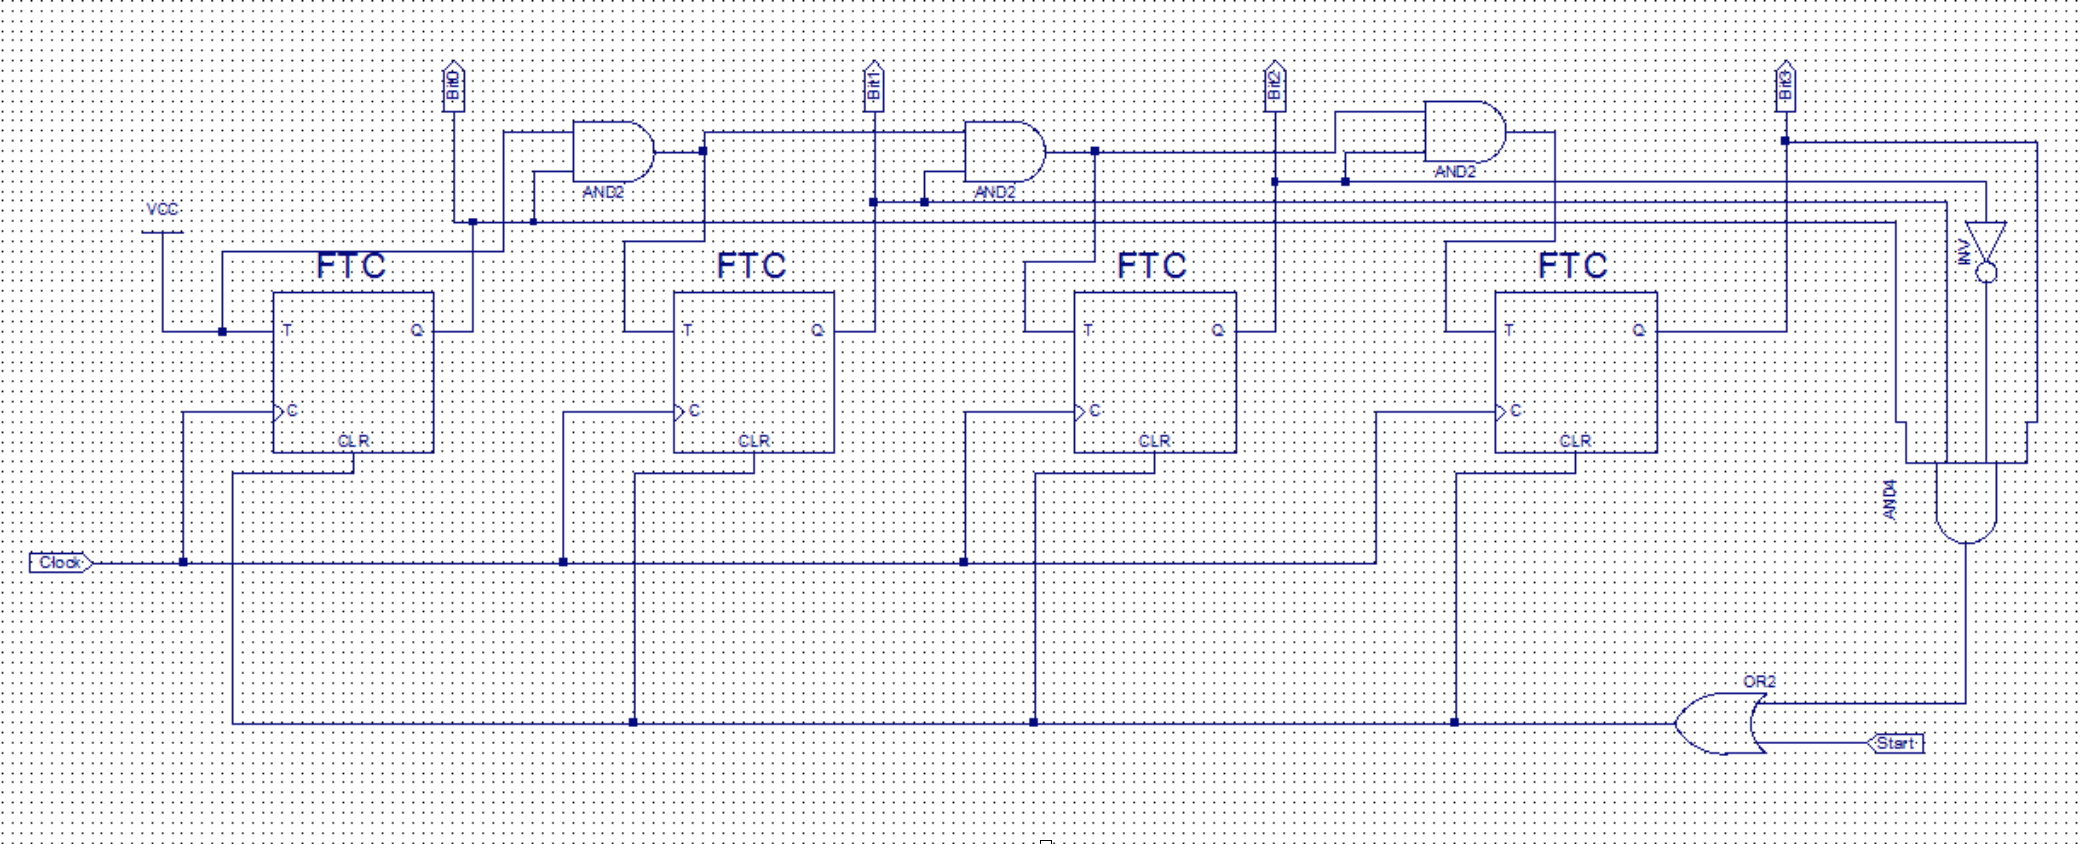
\includegraphics[width=13.5cm]{schemat.png}
\caption{Schemat układu}
\label{fig:schemat}
\end{figure}

Kolejnym etapem było wygenerowanie pliku VHDL oraz zmodyfikowanie go w taki sposób, aby odpowiadał naszym potrzebom.

\begin{listing}[H]
\caption{Kod VHDL}
\begin{minted}[linenos,breaklines]{vhdl}
LIBRARY ieee; 
USE ieee.std_logic_1164.ALL; 
USE ieee.numeric_std.ALL; 
LIBRARY UNISIM; 
USE UNISIM.Vcomponents.ALL; 
ENTITY Lab1Schema_Lab1Schema_sch_tb IS 
END Lab1Schema_Lab1Schema_sch_tb; 
ARCHITECTURE behavioral OF Lab1Schema_Lab1Schema_sch_tb IS  
 
  
 
  COMPONENT Lab1Schema 
   PORT( Bit0:OUTSTD_LOGIC;  
          Bit1:OUTSTD_LOGIC;  
          Bit2:OUTSTD_LOGIC;  
          Clock:INSTD_LOGIC;  
          Bit3:OUTSTD_LOGIC;  
          Start:INSTD_LOGIC); 
   END COMPONENT; 
 
   SIGNAL Bit0:STD_LOGIC; 
   SIGNAL Bit1:STD_LOGIC; 
   SIGNAL Bit2:STD_LOGIC; 
   SIGNAL Clock:STD_LOGIC :='0'; 
   SIGNAL Bit3:STD_LOGIC; 
   SIGNAL Start:STD_LOGIC; 
 
BEGIN 
 
   UUT: Lab1Schema PORT MAP( 
Bit0 => Bit0,  
Bit1 => Bit1,  
Bit2 => Bit2,  
Clock => Clock,  
Bit3 => Bit3,  
Start => Start 
   ); 
 
   Start <= '1', '0' after 100 ns; 
   Clock <= not Clock after 500 ns; 
 
END; 
\end{minted}
\end{listing}

\begin{itemize}
    \item Bit0 -- Bit3 to kolejne wyjścia układu (Bit0 to najmłodszy bit, a Bit3 najstarszy).
    \item Clock to wejście układu odpowiadające za dostarczenie sygnału zegara.
    \item Start to wejście układu odpowiadające za początkowy sygnał zerujący wszystkie przerzutniki.
\end{itemize}
Następnym zadaniem, które wykonaliśmy było skompilowanie układu oraz uruchomienie go w symulatorze.  

\begin{figure}[H]
\centering
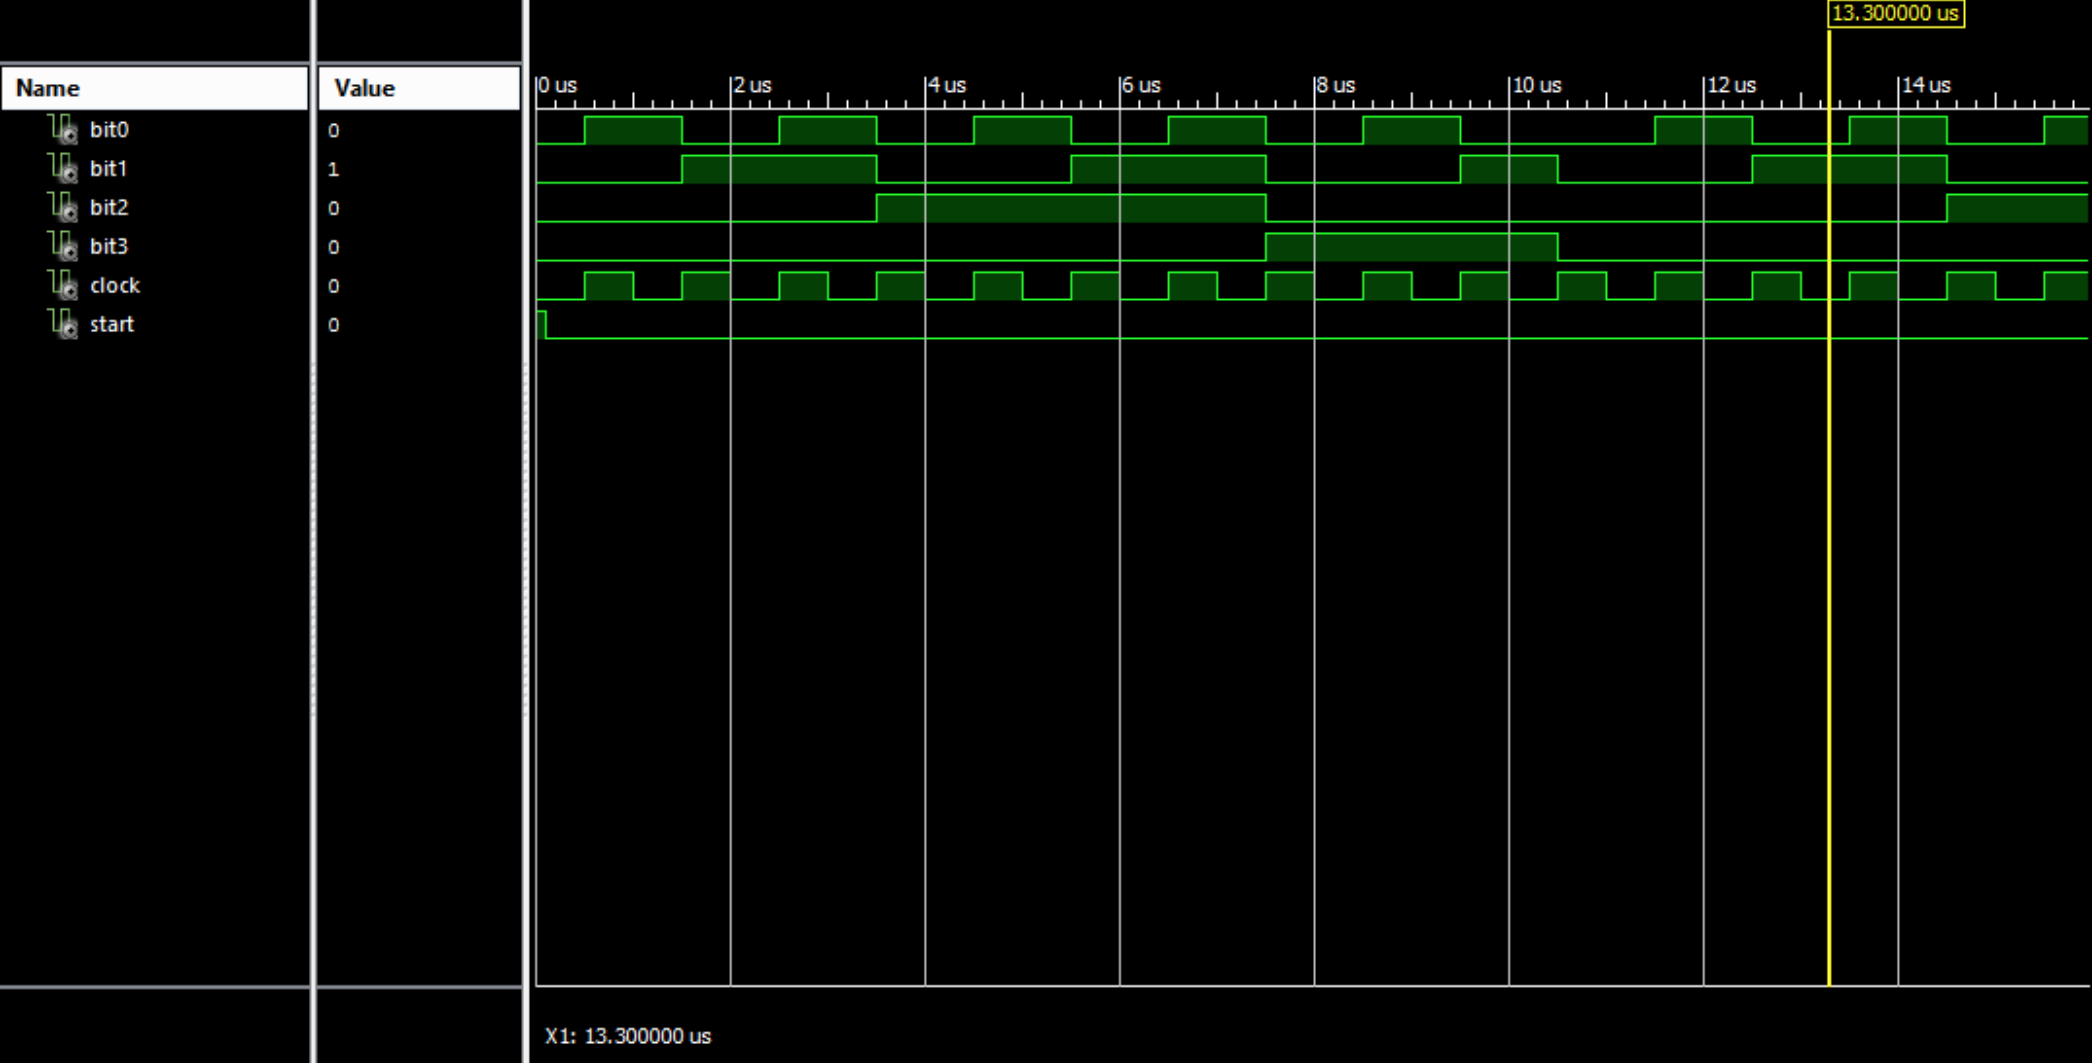
\includegraphics[width=13.5cm]{symulacja.png}
\caption{Schemat układu}
\label{fig:symulacja}
\end{figure}
Symulacja pokazuje, że zaprojektowany przez nas układ działa poprawnie.
\\\\
Ostatnie zadanie polegało na wygenerowaniu pliku .jed, który jest używany do programowania mikroprocesorów. Następnie przesłaliśmy nasz program na płytkę, gdzie po negacji bitów wyjściowych licznik w poprawny sposób odliczał wartości z przedziału od 1 do 10.

\section{Wnioski}
Podczas laboratoriów mogliśmy zapoznać się z podstawami tworzenia oprogramowania w programie ISE Design Suite. Dowiedzieliśmy się jak przeprowadzać symulacje oraz przesyłać wykonany przez nas program na płytkę.
\end{document}